%
% File emnlp2020.tex
%
%% Based on the style files for ACL 2020, which were
%% Based on the style files for ACL 2018, NAACL 2018/19, which were
%% Based on the style files for ACL-2015, with some improvements
%%  taken from the NAACL-2016 style
%% Based on the style files for ACL-2014, which were, in turn,
%% based on ACL-2013, ACL-2012, ACL-2011, ACL-2010, ACL-IJCNLP-2009,
%% EACL-2009, IJCNLP-2008...
%% Based on the style files for EACL 2006 by 
%%e.agirre@ehu.es or Sergi.Balari@uab.es
%% and that of ACL 08 by Joakim Nivre and Noah Smith

\documentclass[11pt,a4paper]{article}
\usepackage[hyperref]{emnlp2020}
\usepackage{times}
\usepackage{latexsym}
\renewcommand{\UrlFont}{\ttfamily\small}

% This is not strictly necessary, and may be commented out,
% but it will improve the layout of the manuscript,
% and will typically save some space.
\usepackage{microtype}

\usepackage{mystyle}
\usepackage{subcaption} 

% trellis
\usepackage{tikz}%

\usepackage{algorithm}
\usepackage[noend]{algpseudocode}

\usepackage{pgfplots}

%% ADD BACK!!!!!!!!!!!!!!!!!
%\aclfinalcopy % Uncomment this line for the final submission
%\def\aclpaperid{***} %  Enter the acl Paper ID here

%\setlength\titlebox{5cm}
% You can expand the titlebox if you need extra space
% to show all the authors. Please do not make the titlebox
% smaller than 5cm (the original size); we will check this
% in the camera-ready version and ask you to change it back.

\newcommand\BibTeX{B\textsc{ib}\TeX}
\newcommand\Emit{\mathbf{O}}
\newcommand\Trans{\mathbf{T}}

\title{Scaling Hidden Markov Language Models}

\author{Who Me \\
  Affiliation / Address line 1 \\
  Affiliation / Address line 2 \\
  Affiliation / Address line 3 \\
  \texttt{email@domain} \\\And
  No You \\
  Affiliation / Address line 1 \\
  Affiliation / Address line 2 \\
  Affiliation / Address line 3 \\
  \texttt{email@domain} \\}

\date{}

\begin{document}
\maketitle
\begin{abstract}
The hidden Markov model (HMM) is a fundamental tool for sequence modeling that 
cleanly separates the hidden state from the emission structure.
However, this clean separation makes HMMs difficult to fit to large datasets in modern NLP, 
and they have fallen out of use due to very poor performance 
compared to fully observed models. This work revisits the challenge of 
scaling HMMs to language modeling datasets, taking ideas from recent approaches to neural modeling.
We propose methods for scaling HMMs to massive state spaces, while maintaining compact parameterization, effective regularization, and efficient exact inference. Experiments show that this approach leads to models that are much more accurate than previous HMMs and ngram-based methods while nearing the performance of NN models. 
\end{abstract}

\section{Introduction}


% Hidden Markov models are classic models that have been abandoned.
Hidden Markov models (HMMs) are a fundamental latent-variable model for sequential data.
%They are core to time-series problems in bioinformatics, reinforcement learning, and,
%of course, natural language processing.
Historically they have been used extensively in NLP for tasks such as
sequence modeling \citep{rabiner1990tut}, alignment \citep{vogel1996hmm},
and even, in a few cases, to language modeling \citep{kuhn1994hmmlm,huang2011thesis}. 
Compared to other approaches for sequence models, HMMs are naturally appealing since they 
fully separate out the process of sequential memory from the process of generation, while allowing for 
exact posterior inference. 

%MMs remain an appealing modeling tool that separates out the facets of discrete model memory from
%the generation of observations. 

%In recent years, most models in 
%For the task of language modeling,
%HMMs were explored in work by \citet{kuhn1994hmmlm,huang2011thesis}
%but were not revisited until recently \citep{krakovna2016hmm,dedieu2019learning}.

State-of-the-art systems in NLP have moved away from utilizing latent hidden states and toward deterministic deep neural models.
%particularly for structured models. For instance in the area of language modeling, systems primarily model observed words using n-gram models, feedforward neural networks \citep{bengio2003nlm}, recurrent neural networks \citep{mikolov2010rnn,zaremba2014lstm,merity2017awdlstm}
%or transformers \citep{radford2019language}.
%This progress has led to the common wisdom that latent-variable models like HMMs are not
%competitive with fully observed models.
We take several lessons from the success of deep neural models for NLP tasks:
(a) the right factorization is critically important for representation learning, e.g. a feedforward model \cite{bengio2003nlm}
can have the same probabilistic structure as an n-gram model while performing significantly better;
(b) overparameterization is critical for finding better local optima,
e.g. overly large LSTMs \cite{zaremba2014lstm} show marked improvements in performance;
(c) regularization choices are necessary to find good solutions for different model parameterizations,
e.g. experiments by \citet{merity2017awdlstm} outline a variety of training choices.

We revisit HMMs for language modeling, positing that competitive performance may just require very large models. 
%To scale to large state-spaces, we need scalable parameterizations, efficient inference, and  effective regularization.
We develop a neural parameterization for HMMs that extends 
them to comparable size and structure of deep models.
We combine this parameterization with a modeling constraint that allows us to utilize HMMs with very large state spaces,
while maintaining efficient exact inference.
Finally we incorporate a variant of dropout that both improves accuracy
and reduces the computational overhead by an order of magnitude during training. 

Experiments employ VL-HMMs on two language modeling datasets. We find that our HMM extension significantly outperforms past HMMs as well as n-gram models. 
It also performs comparably to neural counterparts with a similar number of parameters
while maintaining uncertainty over the state dynamics.

\section{Related Work}

Several recent papers have combined HMMs with 
neural networks. \citet{buys2018hmm}
develop an approach to relax the HMM with results that either have HMM performance much worse than
an n-gram model or require altering the probabilistic structure.  \citet{krakovna2016hmm} utilize model combination with a recurrent neural network to connect both approaches in a 20 state model. We demonstrate how to scale to orders of magnitude more states and show performance surpassing n-gram models.

% Prior work has tried neural parameterizations, but with small state spaces.
Prior work has demonstrated the benefits of neural parameterization of structured generative models. 
For HMMs, \citet{tran2016hmm} demonstrate improvements in POS induction with a
neural parameterization of an HMM.
Other work has used neural parameterization for classic models, such as 
dependency models with valence \citep{han2017dependency},
hidden semi-Markov models \citep{wiseman2018hsmm},
and context free grammars \citep{kim2019cpcfg}.
All of these works use latent variables with relatively small state spaces,
as the goal of both was structure induction rather than language modeling itself.
We extend the neural parameterization with the aim of supervised modeling.

% Prior work has tried large state spaces with scalar parameterizations.
\begin{comment}
We also draw inspiration from the experiments with
cloned HMMs by \citet{dedieu2019learning},
who propose to introduce sparsity constraints in scalar
emission distribution of HMMs in order to make conditional inference
tractable in large state spaces.
They train a 30k state HMM on character-level language modeling
by constraining every state to emit only a single character type.
This particular constraint is problematic for language modeling at the word level,
where the vocabulary size is much larger.
We build on their work by proposing a sparsity constraint based on
Brown clustering \citep{brown1992} which allows us to extend their
work to vocabularies that are larger than the state space.
\end{comment}


% State splitting / refinement
Finally, another approach to scaling to larger state spaces is to initialize
with a small state space then grow the state space via a split-merge process
\citep{petrov2006splitmerge,huang2011thesis}.
In particular, \citet{huang2011thesis} learn an HMM for language modeling
via this process.
%Additionally, the cloned HMM \citep{dedieu2019learning} can be seen
%as an HMM that starts with a single state per word,
%then splits every state into $k$ states at the start
%with no subsequent splits or merges.
The application of more complicated split-merge
procedures is an avenue for future work,
as we focus on fixed-size state spaces.

%There are also extensions of HMMs, such as factorial HMMs \cite{zoubin1997fhmm,nepal2013fhmm}
%and context free grammars \citep{kim2019cpcfg}.
%We leave scaling more expressive models to large state spaces for future work,
%and focus on scaling the basic HMM.

\begin{comment}
\begin{figure}[t]
\centering
\begin{tikzpicture}[]
\node[latent] (z0) {$z_0$} ;
\node[latent] (z1) [right=1.25cm of z0] {$z_1$} ;
\node[latent] (z2) [right=1.25cm of z1] {$z_2$} ;
%\node (dots) [right=1.25cm of z2] {$\cdots$} ;
%\node[latent] (zt) [right=1.25cm of dots] {$z_T$} ;

\node[obs]    (x0) [below = 0.75cm of z0] {$x_0$};
\node[obs]    (x1) [below = 0.75cm of z1] {$x_1$};
\node[obs]    (x2) [below = 0.75cm of z2] {$x_2$};
%\node (adots) [right=1.25cm of x2] {$$} ;
%\node[latent] (xt) [right=1.25cm of adots] {$x_T$} ;

\edge {z0} {x0};
\edge {z1} {x1};
\edge {z2} {x2};
\edge {z0} {z1};
\edge {z1} {z2};
%\edge {z2} {zt};
%\edge {dots} {zt};

\end{tikzpicture}

\caption{
\label{fig:hmm}
An HMM with tokens $x_t$ and states $z_t$.
}
\end{figure}
\end{comment}

\section{Background: HMMs}

We are interested in learning a distribution over observed tokens
$\bx = \langle x_1, \ldots, x_T \rangle$, with each token $x_t$
an element of the finite vocabulary $\mcX$.
Hidden Markov models (HMMs) specify a joint distribution over 
observed tokens $\bx$ and discrete latent states $\bz = \langle z_1, \ldots, z_T \rangle$,
with each $z_t$ from finite set $\mcZ$.
For notational convenience, we define the starting state $z_0=\epsilon$.
%The model is defined by the following generative process (shown in figure~\ref{fig:hmm}):
%For every time step $t \in \set{0,\ldots,T}$, choose a state given the previous state
%$z_t \mid z_{t-1}$ from the transition distribution $p(z_t \mid z_{t-1})$.
%Then choose a token given the current state $x_t \mid z_t$
%from the emission distribution $p(x_t \mid z_t)$.
This yields the joint distribution
\begin{equation}
p(\bx, \bz; \theta)
= \prod_{t=1}^T p(x_t\mid z_t)p(z_t \mid z_{t-1})
\end{equation}
%By virtue of modeling the joint distribution over $\bx_{0:T},\bz_{0:T}$,
%HMMs maintain uncertainty over both observed words the unobserved latent states.
%Contrast this with another class of language models, recurrent neural networks (RNNs),
%which only maintain uncertainty over the observed $\bx_{0:T}$.
%At every timestep $t$, the generative process bottlenecks all information from the past
%through a single discrete state $z_t$ from a finite set.
%This contrasts 
\noindent The distributions are parameterized as follows
\begin{equation}
\label{param}
%p(z_1 | z_0) &\propto e^{\psi_{z_1}}\\
 p(z_t \mid z_{t-1}) \propto e^{\psi_{z_tz_{t-1}}} \; \ p(x_t \mid z_t) \propto e^{\phi_{x_tz_t}}
\end{equation}
with  transitions $\psi \in \mathbb{R}^{|\mcZ|\times|\mcZ|}$
and  emissions $\phi \in \mathbb{R}^{|\mcX| \times |\mcZ|}$.
We refer to 
$p(z_t \mid z_{t-1})$ as $\mathbf{T}$ and $p(x_t \mid z_t)$ as $\mathbf{O}$.

We distinguish two types of parameterizations: \textit{scalar} and \textit{neural}.
A scalar parameterization simply uses $\theta = \set{\phi,\psi}$ to fit one model parameter for
each distributional parameter ($O(|\mcZ|^2 + |\mcX||\mcZ|)$ model parameters). A neural parameterization uses $\theta$ as the parameters of a neural network
that generates $\phi$ and $\psi$ for the distribution, which allow for task based factorization. 

In order to fit an HMM to data $\bx$,
we must marginalize over the latent states to obtain the likelihood
$p(\bx) = \sum_{\bz}p(\bx,\bz)$.
This sum can be computed in time $O(T|\mcZ|^2)$ via dynamic programming,
which becomes prohibitive if the number of latent states $|\mcZ|$ is large.
We can then optimize the likelihood 
with gradient ascent (or alternative variants of expectation maximization).

%\footnote{An alternative method would be to employ expectation maximization,
%however there is no closed form solution for the M-step with a neural parameterization.
%Gradient ascent is applicable to both the scalar and neural parameterizations.}

\noindent \textbf{HMMs and RNNs}
% Motivate HMMs over RNNs.
% Simplicity.
% Faithful to generative process.
% Computational reasons.
%Recurrent neural networks (RNNs) %are one of the main alternatives to HMMs,
%also model data with sequential structure and often achieve stronger performance. 
%HMMs though are a useful alternative approach. 
Recurrent neural networks (RNNs) do not attempt to decouple the latent dynamics from the observed.
This often leads to improved accuracy,
but does not allow for posterior inference or for directly incorporating additional
state information.
A further benefit of HMMs is that, unlike RNNs,
their associative structure allows for parallel inference
via the prefix-sum algorithm \cite{ladner1980prefix}.\footnote{Quasi-RNNs \citep{bradbury2016qrnn} also have a logarithmic dependency on $T$
by applying the same prefix-sum trick, but do not model uncertainty over
latent dynamics.}

%Our approach starts by defining two partitions:
%one for the hidden states $\pi: \mcZ \to [m]$,
%where $m$ is the number of partitions and each $|\pi(z)| = k, \forall z$;
%and one for the observations $\sigma: \mcX \to [m]$.
%Given the structure defined by $\pi$ and $\sigma$, we build models with large
%capacity that admit tractable inference.

\section{Scaling HMMs}

\begin{figure}[!t]
\begin{center}
\normalsize%
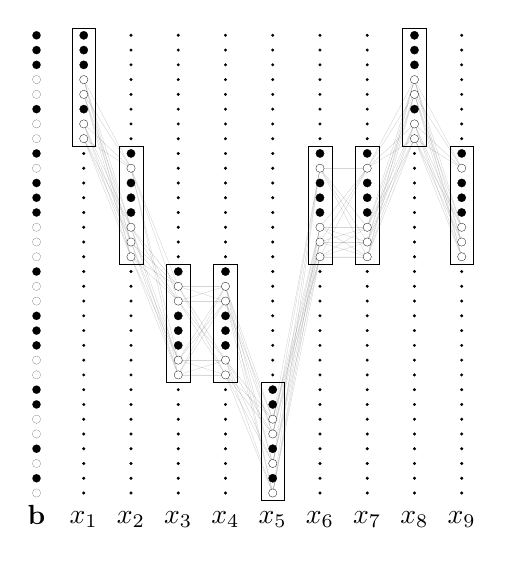
\begin{tikzpicture}%
\path[draw,line width=0.01pt,fill=white,radius=1.5pt] (0.0,0.0) circle;%
\path[draw,line width=0.01pt,fill=black,radius=1.5pt] (0.0,0.1875) circle;%
\path[draw,line width=0.01pt,fill=white,radius=1.5pt] (0.0,0.375) circle;%
\path[draw,line width=0.01pt,fill=black,radius=1.5pt] (0.0,0.5625) circle;%
\path[draw,line width=0.01pt,fill=white,radius=1.5pt] (0.0,0.75) circle;%
\path[draw,line width=0.01pt,fill=white,radius=1.5pt] (0.0,0.9375) circle;%
\path[draw,line width=0.01pt,fill=black,radius=1.5pt] (0.0,1.125) circle;%
\path[draw,line width=0.01pt,fill=black,radius=1.5pt] (0.0,1.3125) circle;%
\path[draw,line width=0.01pt,fill=white,radius=1.5pt] (0.0,1.5) circle;%
\path[draw,line width=0.01pt,fill=white,radius=1.5pt] (0.0,1.6875) circle;%
\path[draw,line width=0.01pt,fill=black,radius=1.5pt] (0.0,1.875) circle;%
\path[draw,line width=0.01pt,fill=black,radius=1.5pt] (0.0,2.0625) circle;%
\path[draw,line width=0.01pt,fill=black,radius=1.5pt] (0.0,2.25) circle;%
\path[draw,line width=0.01pt,fill=white,radius=1.5pt] (0.0,2.4375) circle;%
\path[draw,line width=0.01pt,fill=white,radius=1.5pt] (0.0,2.625) circle;%
\path[draw,line width=0.01pt,fill=black,radius=1.5pt] (0.0,2.8125) circle;%
\path[draw,line width=0.01pt,fill=white,radius=1.5pt] (0.0,3.0) circle;%
\path[draw,line width=0.01pt,fill=white,radius=1.5pt] (0.0,3.1875) circle;%
\path[draw,line width=0.01pt,fill=white,radius=1.5pt] (0.0,3.375) circle;%
\path[draw,line width=0.01pt,fill=black,radius=1.5pt] (0.0,3.5625) circle;%
\path[draw,line width=0.01pt,fill=black,radius=1.5pt] (0.0,3.75) circle;%
\path[draw,line width=0.01pt,fill=black,radius=1.5pt] (0.0,3.9375) circle;%
\path[draw,line width=0.01pt,fill=white,radius=1.5pt] (0.0,4.125) circle;%
\path[draw,line width=0.01pt,fill=black,radius=1.5pt] (0.0,4.3125) circle;%
\path[draw,line width=0.01pt,fill=white,radius=1.5pt] (0.0,4.5) circle;%
\path[draw,line width=0.01pt,fill=white,radius=1.5pt] (0.0,4.6875) circle;%
\path[draw,line width=0.01pt,fill=black,radius=1.5pt] (0.0,4.875) circle;%
\path[draw,line width=0.01pt,fill=white,radius=1.5pt] (0.0,5.0625) circle;%
\path[draw,line width=0.01pt,fill=white,radius=1.5pt] (0.0,5.25) circle;%
\path[draw,line width=0.01pt,fill=black,radius=1.5pt] (0.0,5.4375) circle;%
\path[draw,line width=0.01pt,fill=black,radius=1.5pt] (0.0,5.625) circle;%
\path[draw,line width=0.01pt,fill=black,radius=1.5pt] (0.0,5.8125) circle;%
\path[draw,line width=0.1pt,opacity=0.15,fill=black] (0.6,4.5) -- (1.2,3.0);%
\path[draw,line width=0.1pt,opacity=0.15,fill=black] (0.6,4.5) -- (1.2,3.1875);%
\path[draw,line width=0.1pt,opacity=0.15,fill=black] (0.6,4.5) -- (1.2,3.375);%
\path[draw,line width=0.1pt,opacity=0.15,fill=black] (0.6,4.5) -- (1.2,4.125);%
\path[draw,line width=0.1pt,opacity=0.15,fill=black] (0.6,4.6875) -- (1.2,3.0);%
\path[draw,line width=0.1pt,opacity=0.15,fill=black] (0.6,4.6875) -- (1.2,3.1875);%
\path[draw,line width=0.1pt,opacity=0.15,fill=black] (0.6,4.6875) -- (1.2,3.375);%
\path[draw,line width=0.1pt,opacity=0.15,fill=black] (0.6,4.6875) -- (1.2,4.125);%
\path[draw,line width=0.1pt,opacity=0.15,fill=black] (0.6,5.0625) -- (1.2,3.0);%
\path[draw,line width=0.1pt,opacity=0.15,fill=black] (0.6,5.0625) -- (1.2,3.1875);%
\path[draw,line width=0.1pt,opacity=0.15,fill=black] (0.6,5.0625) -- (1.2,3.375);%
\path[draw,line width=0.1pt,opacity=0.15,fill=black] (0.6,5.0625) -- (1.2,4.125);%
\path[draw,line width=0.1pt,opacity=0.15,fill=black] (0.6,5.25) -- (1.2,3.0);%
\path[draw,line width=0.1pt,opacity=0.15,fill=black] (0.6,5.25) -- (1.2,3.1875);%
\path[draw,line width=0.1pt,opacity=0.15,fill=black] (0.6,5.25) -- (1.2,3.375);%
\path[draw,line width=0.1pt,opacity=0.15,fill=black] (0.6,5.25) -- (1.2,4.125);%
\path[draw,line width=0.1pt,opacity=0.15,fill=black] (1.2,3.0) -- (1.8,1.5);%
\path[draw,line width=0.1pt,opacity=0.15,fill=black] (1.2,3.0) -- (1.8,1.6875);%
\path[draw,line width=0.1pt,opacity=0.15,fill=black] (1.2,3.0) -- (1.8,2.4375);%
\path[draw,line width=0.1pt,opacity=0.15,fill=black] (1.2,3.0) -- (1.8,2.625);%
\path[draw,line width=0.1pt,opacity=0.15,fill=black] (1.2,3.1875) -- (1.8,1.5);%
\path[draw,line width=0.1pt,opacity=0.15,fill=black] (1.2,3.1875) -- (1.8,1.6875);%
\path[draw,line width=0.1pt,opacity=0.15,fill=black] (1.2,3.1875) -- (1.8,2.4375);%
\path[draw,line width=0.1pt,opacity=0.15,fill=black] (1.2,3.1875) -- (1.8,2.625);%
\path[draw,line width=0.1pt,opacity=0.15,fill=black] (1.2,3.375) -- (1.8,1.5);%
\path[draw,line width=0.1pt,opacity=0.15,fill=black] (1.2,3.375) -- (1.8,1.6875);%
\path[draw,line width=0.1pt,opacity=0.15,fill=black] (1.2,3.375) -- (1.8,2.4375);%
\path[draw,line width=0.1pt,opacity=0.15,fill=black] (1.2,3.375) -- (1.8,2.625);%
\path[draw,line width=0.1pt,opacity=0.15,fill=black] (1.2,4.125) -- (1.8,1.5);%
\path[draw,line width=0.1pt,opacity=0.15,fill=black] (1.2,4.125) -- (1.8,1.6875);%
\path[draw,line width=0.1pt,opacity=0.15,fill=black] (1.2,4.125) -- (1.8,2.4375);%
\path[draw,line width=0.1pt,opacity=0.15,fill=black] (1.2,4.125) -- (1.8,2.625);%
\path[draw,line width=0.1pt,opacity=0.15,fill=black] (1.8,1.5) -- (2.4,1.5);%
\path[draw,line width=0.1pt,opacity=0.15,fill=black] (1.8,1.5) -- (2.4,1.6875);%
\path[draw,line width=0.1pt,opacity=0.15,fill=black] (1.8,1.5) -- (2.4,2.4375);%
\path[draw,line width=0.1pt,opacity=0.15,fill=black] (1.8,1.5) -- (2.4,2.625);%
\path[draw,line width=0.1pt,opacity=0.15,fill=black] (1.8,1.6875) -- (2.4,1.5);%
\path[draw,line width=0.1pt,opacity=0.15,fill=black] (1.8,1.6875) -- (2.4,1.6875);%
\path[draw,line width=0.1pt,opacity=0.15,fill=black] (1.8,1.6875) -- (2.4,2.4375);%
\path[draw,line width=0.1pt,opacity=0.15,fill=black] (1.8,1.6875) -- (2.4,2.625);%
\path[draw,line width=0.1pt,opacity=0.15,fill=black] (1.8,2.4375) -- (2.4,1.5);%
\path[draw,line width=0.1pt,opacity=0.15,fill=black] (1.8,2.4375) -- (2.4,1.6875);%
\path[draw,line width=0.1pt,opacity=0.15,fill=black] (1.8,2.4375) -- (2.4,2.4375);%
\path[draw,line width=0.1pt,opacity=0.15,fill=black] (1.8,2.4375) -- (2.4,2.625);%
\path[draw,line width=0.1pt,opacity=0.15,fill=black] (1.8,2.625) -- (2.4,1.5);%
\path[draw,line width=0.1pt,opacity=0.15,fill=black] (1.8,2.625) -- (2.4,1.6875);%
\path[draw,line width=0.1pt,opacity=0.15,fill=black] (1.8,2.625) -- (2.4,2.4375);%
\path[draw,line width=0.1pt,opacity=0.15,fill=black] (1.8,2.625) -- (2.4,2.625);%
\path[draw,line width=0.1pt,opacity=0.15,fill=black] (2.4,1.5) -- (3.0,0.0);%
\path[draw,line width=0.1pt,opacity=0.15,fill=black] (2.4,1.5) -- (3.0,0.375);%
\path[draw,line width=0.1pt,opacity=0.15,fill=black] (2.4,1.5) -- (3.0,0.75);%
\path[draw,line width=0.1pt,opacity=0.15,fill=black] (2.4,1.5) -- (3.0,0.9375);%
\path[draw,line width=0.1pt,opacity=0.15,fill=black] (2.4,1.6875) -- (3.0,0.0);%
\path[draw,line width=0.1pt,opacity=0.15,fill=black] (2.4,1.6875) -- (3.0,0.375);%
\path[draw,line width=0.1pt,opacity=0.15,fill=black] (2.4,1.6875) -- (3.0,0.75);%
\path[draw,line width=0.1pt,opacity=0.15,fill=black] (2.4,1.6875) -- (3.0,0.9375);%
\path[draw,line width=0.1pt,opacity=0.15,fill=black] (2.4,2.4375) -- (3.0,0.0);%
\path[draw,line width=0.1pt,opacity=0.15,fill=black] (2.4,2.4375) -- (3.0,0.375);%
\path[draw,line width=0.1pt,opacity=0.15,fill=black] (2.4,2.4375) -- (3.0,0.75);%
\path[draw,line width=0.1pt,opacity=0.15,fill=black] (2.4,2.4375) -- (3.0,0.9375);%
\path[draw,line width=0.1pt,opacity=0.15,fill=black] (2.4,2.625) -- (3.0,0.0);%
\path[draw,line width=0.1pt,opacity=0.15,fill=black] (2.4,2.625) -- (3.0,0.375);%
\path[draw,line width=0.1pt,opacity=0.15,fill=black] (2.4,2.625) -- (3.0,0.75);%
\path[draw,line width=0.1pt,opacity=0.15,fill=black] (2.4,2.625) -- (3.0,0.9375);%
\path[draw,line width=0.1pt,opacity=0.15,fill=black] (3.0,0.0) -- (3.6,3.0);%
\path[draw,line width=0.1pt,opacity=0.15,fill=black] (3.0,0.0) -- (3.6,3.1875);%
\path[draw,line width=0.1pt,opacity=0.15,fill=black] (3.0,0.0) -- (3.6,3.375);%
\path[draw,line width=0.1pt,opacity=0.15,fill=black] (3.0,0.0) -- (3.6,4.125);%
\path[draw,line width=0.1pt,opacity=0.15,fill=black] (3.0,0.375) -- (3.6,3.0);%
\path[draw,line width=0.1pt,opacity=0.15,fill=black] (3.0,0.375) -- (3.6,3.1875);%
\path[draw,line width=0.1pt,opacity=0.15,fill=black] (3.0,0.375) -- (3.6,3.375);%
\path[draw,line width=0.1pt,opacity=0.15,fill=black] (3.0,0.375) -- (3.6,4.125);%
\path[draw,line width=0.1pt,opacity=0.15,fill=black] (3.0,0.75) -- (3.6,3.0);%
\path[draw,line width=0.1pt,opacity=0.15,fill=black] (3.0,0.75) -- (3.6,3.1875);%
\path[draw,line width=0.1pt,opacity=0.15,fill=black] (3.0,0.75) -- (3.6,3.375);%
\path[draw,line width=0.1pt,opacity=0.15,fill=black] (3.0,0.75) -- (3.6,4.125);%
\path[draw,line width=0.1pt,opacity=0.15,fill=black] (3.0,0.9375) -- (3.6,3.0);%
\path[draw,line width=0.1pt,opacity=0.15,fill=black] (3.0,0.9375) -- (3.6,3.1875);%
\path[draw,line width=0.1pt,opacity=0.15,fill=black] (3.0,0.9375) -- (3.6,3.375);%
\path[draw,line width=0.1pt,opacity=0.15,fill=black] (3.0,0.9375) -- (3.6,4.125);%
\path[draw,line width=0.1pt,opacity=0.15,fill=black] (3.6,3.0) -- (4.2,3.0);%
\path[draw,line width=0.1pt,opacity=0.15,fill=black] (3.6,3.0) -- (4.2,3.1875);%
\path[draw,line width=0.1pt,opacity=0.15,fill=black] (3.6,3.0) -- (4.2,3.375);%
\path[draw,line width=0.1pt,opacity=0.15,fill=black] (3.6,3.0) -- (4.2,4.125);%
\path[draw,line width=0.1pt,opacity=0.15,fill=black] (3.6,3.1875) -- (4.2,3.0);%
\path[draw,line width=0.1pt,opacity=0.15,fill=black] (3.6,3.1875) -- (4.2,3.1875);%
\path[draw,line width=0.1pt,opacity=0.15,fill=black] (3.6,3.1875) -- (4.2,3.375);%
\path[draw,line width=0.1pt,opacity=0.15,fill=black] (3.6,3.1875) -- (4.2,4.125);%
\path[draw,line width=0.1pt,opacity=0.15,fill=black] (3.6,3.375) -- (4.2,3.0);%
\path[draw,line width=0.1pt,opacity=0.15,fill=black] (3.6,3.375) -- (4.2,3.1875);%
\path[draw,line width=0.1pt,opacity=0.15,fill=black] (3.6,3.375) -- (4.2,3.375);%
\path[draw,line width=0.1pt,opacity=0.15,fill=black] (3.6,3.375) -- (4.2,4.125);%
\path[draw,line width=0.1pt,opacity=0.15,fill=black] (3.6,4.125) -- (4.2,3.0);%
\path[draw,line width=0.1pt,opacity=0.15,fill=black] (3.6,4.125) -- (4.2,3.1875);%
\path[draw,line width=0.1pt,opacity=0.15,fill=black] (3.6,4.125) -- (4.2,3.375);%
\path[draw,line width=0.1pt,opacity=0.15,fill=black] (3.6,4.125) -- (4.2,4.125);%
\path[draw,line width=0.1pt,opacity=0.15,fill=black] (4.2,3.0) -- (4.8,4.5);%
\path[draw,line width=0.1pt,opacity=0.15,fill=black] (4.2,3.0) -- (4.8,4.6875);%
\path[draw,line width=0.1pt,opacity=0.15,fill=black] (4.2,3.0) -- (4.8,5.0625);%
\path[draw,line width=0.1pt,opacity=0.15,fill=black] (4.2,3.0) -- (4.8,5.25);%
\path[draw,line width=0.1pt,opacity=0.15,fill=black] (4.2,3.1875) -- (4.8,4.5);%
\path[draw,line width=0.1pt,opacity=0.15,fill=black] (4.2,3.1875) -- (4.8,4.6875);%
\path[draw,line width=0.1pt,opacity=0.15,fill=black] (4.2,3.1875) -- (4.8,5.0625);%
\path[draw,line width=0.1pt,opacity=0.15,fill=black] (4.2,3.1875) -- (4.8,5.25);%
\path[draw,line width=0.1pt,opacity=0.15,fill=black] (4.2,3.375) -- (4.8,4.5);%
\path[draw,line width=0.1pt,opacity=0.15,fill=black] (4.2,3.375) -- (4.8,4.6875);%
\path[draw,line width=0.1pt,opacity=0.15,fill=black] (4.2,3.375) -- (4.8,5.0625);%
\path[draw,line width=0.1pt,opacity=0.15,fill=black] (4.2,3.375) -- (4.8,5.25);%
\path[draw,line width=0.1pt,opacity=0.15,fill=black] (4.2,4.125) -- (4.8,4.5);%
\path[draw,line width=0.1pt,opacity=0.15,fill=black] (4.2,4.125) -- (4.8,4.6875);%
\path[draw,line width=0.1pt,opacity=0.15,fill=black] (4.2,4.125) -- (4.8,5.0625);%
\path[draw,line width=0.1pt,opacity=0.15,fill=black] (4.2,4.125) -- (4.8,5.25);%
\path[draw,line width=0.1pt,opacity=0.15,fill=black] (4.8,4.5) -- (5.4,3.0);%
\path[draw,line width=0.1pt,opacity=0.15,fill=black] (4.8,4.5) -- (5.4,3.1875);%
\path[draw,line width=0.1pt,opacity=0.15,fill=black] (4.8,4.5) -- (5.4,3.375);%
\path[draw,line width=0.1pt,opacity=0.15,fill=black] (4.8,4.5) -- (5.4,4.125);%
\path[draw,line width=0.1pt,opacity=0.15,fill=black] (4.8,4.6875) -- (5.4,3.0);%
\path[draw,line width=0.1pt,opacity=0.15,fill=black] (4.8,4.6875) -- (5.4,3.1875);%
\path[draw,line width=0.1pt,opacity=0.15,fill=black] (4.8,4.6875) -- (5.4,3.375);%
\path[draw,line width=0.1pt,opacity=0.15,fill=black] (4.8,4.6875) -- (5.4,4.125);%
\path[draw,line width=0.1pt,opacity=0.15,fill=black] (4.8,5.0625) -- (5.4,3.0);%
\path[draw,line width=0.1pt,opacity=0.15,fill=black] (4.8,5.0625) -- (5.4,3.1875);%
\path[draw,line width=0.1pt,opacity=0.15,fill=black] (4.8,5.0625) -- (5.4,3.375);%
\path[draw,line width=0.1pt,opacity=0.15,fill=black] (4.8,5.0625) -- (5.4,4.125);%
\path[draw,line width=0.1pt,opacity=0.15,fill=black] (4.8,5.25) -- (5.4,3.0);%
\path[draw,line width=0.1pt,opacity=0.15,fill=black] (4.8,5.25) -- (5.4,3.1875);%
\path[draw,line width=0.1pt,opacity=0.15,fill=black] (4.8,5.25) -- (5.4,3.375);%
\path[draw,line width=0.1pt,opacity=0.15,fill=black] (4.8,5.25) -- (5.4,4.125);%
\path[draw,line width=0.2pt] (0.45,4.40625) rectangle (0.75,5.90625);%
\path[draw,line width=0.2pt] (1.05,2.90625) rectangle (1.35,4.40625);%
\path[draw,line width=0.2pt] (1.65,1.40625) rectangle (1.95,2.90625);%
\path[draw,line width=0.2pt] (2.25,1.40625) rectangle (2.55,2.90625);%
\path[draw,line width=0.2pt] (2.85,-0.09375) rectangle (3.15,1.40625);%
\path[draw,line width=0.2pt] (3.45,2.90625) rectangle (3.75,4.40625);%
\path[draw,line width=0.2pt] (4.05,2.90625) rectangle (4.35,4.40625);%
\path[draw,line width=0.2pt] (4.65,4.40625) rectangle (4.95,5.90625);%
\path[draw,line width=0.2pt] (5.25,2.90625) rectangle (5.55,4.40625);%
\node[inner sep=0] (b) at (0.0,-0.28125) {$\mathbf{b}$};%
\node (x1) at (0.6,-0.3375) {$x_1$};%
\node (x2) at (1.2,-0.3375) {$x_2$};%
\node (x3) at (1.8,-0.3375) {$x_3$};%
\node (x4) at (2.4,-0.3375) {$x_4$};%
\node (x5) at (3.0,-0.3375) {$x_5$};%
\node (x6) at (3.6,-0.3375) {$x_6$};%
\node (x7) at (4.2,-0.3375) {$x_7$};%
\node (x8) at (4.8,-0.3375) {$x_8$};%
\node (x9) at (5.4,-0.3375) {$x_9$};%
\path[draw,line width=0.1pt,fill=black,radius=0.5pt] (0.6,0.0) circle;%
\path[draw,line width=0.1pt,fill=black,radius=0.5pt] (0.6,0.1875) circle;%
\path[draw,line width=0.1pt,fill=black,radius=0.5pt] (0.6,0.375) circle;%
\path[draw,line width=0.1pt,fill=black,radius=0.5pt] (0.6,0.5625) circle;%
\path[draw,line width=0.1pt,fill=black,radius=0.5pt] (0.6,0.75) circle;%
\path[draw,line width=0.1pt,fill=black,radius=0.5pt] (0.6,0.9375) circle;%
\path[draw,line width=0.1pt,fill=black,radius=0.5pt] (0.6,1.125) circle;%
\path[draw,line width=0.1pt,fill=black,radius=0.5pt] (0.6,1.3125) circle;%
\path[draw,line width=0.1pt,fill=black,radius=0.5pt] (0.6,1.5) circle;%
\path[draw,line width=0.1pt,fill=black,radius=0.5pt] (0.6,1.6875) circle;%
\path[draw,line width=0.1pt,fill=black,radius=0.5pt] (0.6,1.875) circle;%
\path[draw,line width=0.1pt,fill=black,radius=0.5pt] (0.6,2.0625) circle;%
\path[draw,line width=0.1pt,fill=black,radius=0.5pt] (0.6,2.25) circle;%
\path[draw,line width=0.1pt,fill=black,radius=0.5pt] (0.6,2.4375) circle;%
\path[draw,line width=0.1pt,fill=black,radius=0.5pt] (0.6,2.625) circle;%
\path[draw,line width=0.1pt,fill=black,radius=0.5pt] (0.6,2.8125) circle;%
\path[draw,line width=0.1pt,fill=black,radius=0.5pt] (0.6,3.0) circle;%
\path[draw,line width=0.1pt,fill=black,radius=0.5pt] (0.6,3.1875) circle;%
\path[draw,line width=0.1pt,fill=black,radius=0.5pt] (0.6,3.375) circle;%
\path[draw,line width=0.1pt,fill=black,radius=0.5pt] (0.6,3.5625) circle;%
\path[draw,line width=0.1pt,fill=black,radius=0.5pt] (0.6,3.75) circle;%
\path[draw,line width=0.1pt,fill=black,radius=0.5pt] (0.6,3.9375) circle;%
\path[draw,line width=0.1pt,fill=black,radius=0.5pt] (0.6,4.125) circle;%
\path[draw,line width=0.1pt,fill=black,radius=0.5pt] (0.6,4.3125) circle;%
\path[draw,line width=0.1pt,fill=white,radius=1.5pt] (0.6,4.5) circle;%
\path[draw,line width=0.1pt,fill=white,radius=1.5pt] (0.6,4.6875) circle;%
\path[draw,line width=0.1pt,fill=black,radius=1.5pt] (0.6,4.875) circle;%
\path[draw,line width=0.1pt,fill=white,radius=1.5pt] (0.6,5.0625) circle;%
\path[draw,line width=0.1pt,fill=white,radius=1.5pt] (0.6,5.25) circle;%
\path[draw,line width=0.1pt,fill=black,radius=1.5pt] (0.6,5.4375) circle;%
\path[draw,line width=0.1pt,fill=black,radius=1.5pt] (0.6,5.625) circle;%
\path[draw,line width=0.1pt,fill=black,radius=1.5pt] (0.6,5.8125) circle;%
\path[draw,line width=0.1pt,fill=black,radius=0.5pt] (1.2,0.0) circle;%
\path[draw,line width=0.1pt,fill=black,radius=0.5pt] (1.2,0.1875) circle;%
\path[draw,line width=0.1pt,fill=black,radius=0.5pt] (1.2,0.375) circle;%
\path[draw,line width=0.1pt,fill=black,radius=0.5pt] (1.2,0.5625) circle;%
\path[draw,line width=0.1pt,fill=black,radius=0.5pt] (1.2,0.75) circle;%
\path[draw,line width=0.1pt,fill=black,radius=0.5pt] (1.2,0.9375) circle;%
\path[draw,line width=0.1pt,fill=black,radius=0.5pt] (1.2,1.125) circle;%
\path[draw,line width=0.1pt,fill=black,radius=0.5pt] (1.2,1.3125) circle;%
\path[draw,line width=0.1pt,fill=black,radius=0.5pt] (1.2,1.5) circle;%
\path[draw,line width=0.1pt,fill=black,radius=0.5pt] (1.2,1.6875) circle;%
\path[draw,line width=0.1pt,fill=black,radius=0.5pt] (1.2,1.875) circle;%
\path[draw,line width=0.1pt,fill=black,radius=0.5pt] (1.2,2.0625) circle;%
\path[draw,line width=0.1pt,fill=black,radius=0.5pt] (1.2,2.25) circle;%
\path[draw,line width=0.1pt,fill=black,radius=0.5pt] (1.2,2.4375) circle;%
\path[draw,line width=0.1pt,fill=black,radius=0.5pt] (1.2,2.625) circle;%
\path[draw,line width=0.1pt,fill=black,radius=0.5pt] (1.2,2.8125) circle;%
\path[draw,line width=0.1pt,fill=white,radius=1.5pt] (1.2,3.0) circle;%
\path[draw,line width=0.1pt,fill=white,radius=1.5pt] (1.2,3.1875) circle;%
\path[draw,line width=0.1pt,fill=white,radius=1.5pt] (1.2,3.375) circle;%
\path[draw,line width=0.1pt,fill=black,radius=1.5pt] (1.2,3.5625) circle;%
\path[draw,line width=0.1pt,fill=black,radius=1.5pt] (1.2,3.75) circle;%
\path[draw,line width=0.1pt,fill=black,radius=1.5pt] (1.2,3.9375) circle;%
\path[draw,line width=0.1pt,fill=white,radius=1.5pt] (1.2,4.125) circle;%
\path[draw,line width=0.1pt,fill=black,radius=1.5pt] (1.2,4.3125) circle;%
\path[draw,line width=0.1pt,fill=black,radius=0.5pt] (1.2,4.5) circle;%
\path[draw,line width=0.1pt,fill=black,radius=0.5pt] (1.2,4.6875) circle;%
\path[draw,line width=0.1pt,fill=black,radius=0.5pt] (1.2,4.875) circle;%
\path[draw,line width=0.1pt,fill=black,radius=0.5pt] (1.2,5.0625) circle;%
\path[draw,line width=0.1pt,fill=black,radius=0.5pt] (1.2,5.25) circle;%
\path[draw,line width=0.1pt,fill=black,radius=0.5pt] (1.2,5.4375) circle;%
\path[draw,line width=0.1pt,fill=black,radius=0.5pt] (1.2,5.625) circle;%
\path[draw,line width=0.1pt,fill=black,radius=0.5pt] (1.2,5.8125) circle;%
\path[draw,line width=0.1pt,fill=black,radius=0.5pt] (1.8,0.0) circle;%
\path[draw,line width=0.1pt,fill=black,radius=0.5pt] (1.8,0.1875) circle;%
\path[draw,line width=0.1pt,fill=black,radius=0.5pt] (1.8,0.375) circle;%
\path[draw,line width=0.1pt,fill=black,radius=0.5pt] (1.8,0.5625) circle;%
\path[draw,line width=0.1pt,fill=black,radius=0.5pt] (1.8,0.75) circle;%
\path[draw,line width=0.1pt,fill=black,radius=0.5pt] (1.8,0.9375) circle;%
\path[draw,line width=0.1pt,fill=black,radius=0.5pt] (1.8,1.125) circle;%
\path[draw,line width=0.1pt,fill=black,radius=0.5pt] (1.8,1.3125) circle;%
\path[draw,line width=0.1pt,fill=white,radius=1.5pt] (1.8,1.5) circle;%
\path[draw,line width=0.1pt,fill=white,radius=1.5pt] (1.8,1.6875) circle;%
\path[draw,line width=0.1pt,fill=black,radius=1.5pt] (1.8,1.875) circle;%
\path[draw,line width=0.1pt,fill=black,radius=1.5pt] (1.8,2.0625) circle;%
\path[draw,line width=0.1pt,fill=black,radius=1.5pt] (1.8,2.25) circle;%
\path[draw,line width=0.1pt,fill=white,radius=1.5pt] (1.8,2.4375) circle;%
\path[draw,line width=0.1pt,fill=white,radius=1.5pt] (1.8,2.625) circle;%
\path[draw,line width=0.1pt,fill=black,radius=1.5pt] (1.8,2.8125) circle;%
\path[draw,line width=0.1pt,fill=black,radius=0.5pt] (1.8,3.0) circle;%
\path[draw,line width=0.1pt,fill=black,radius=0.5pt] (1.8,3.1875) circle;%
\path[draw,line width=0.1pt,fill=black,radius=0.5pt] (1.8,3.375) circle;%
\path[draw,line width=0.1pt,fill=black,radius=0.5pt] (1.8,3.5625) circle;%
\path[draw,line width=0.1pt,fill=black,radius=0.5pt] (1.8,3.75) circle;%
\path[draw,line width=0.1pt,fill=black,radius=0.5pt] (1.8,3.9375) circle;%
\path[draw,line width=0.1pt,fill=black,radius=0.5pt] (1.8,4.125) circle;%
\path[draw,line width=0.1pt,fill=black,radius=0.5pt] (1.8,4.3125) circle;%
\path[draw,line width=0.1pt,fill=black,radius=0.5pt] (1.8,4.5) circle;%
\path[draw,line width=0.1pt,fill=black,radius=0.5pt] (1.8,4.6875) circle;%
\path[draw,line width=0.1pt,fill=black,radius=0.5pt] (1.8,4.875) circle;%
\path[draw,line width=0.1pt,fill=black,radius=0.5pt] (1.8,5.0625) circle;%
\path[draw,line width=0.1pt,fill=black,radius=0.5pt] (1.8,5.25) circle;%
\path[draw,line width=0.1pt,fill=black,radius=0.5pt] (1.8,5.4375) circle;%
\path[draw,line width=0.1pt,fill=black,radius=0.5pt] (1.8,5.625) circle;%
\path[draw,line width=0.1pt,fill=black,radius=0.5pt] (1.8,5.8125) circle;%
\path[draw,line width=0.1pt,fill=black,radius=0.5pt] (2.4,0.0) circle;%
\path[draw,line width=0.1pt,fill=black,radius=0.5pt] (2.4,0.1875) circle;%
\path[draw,line width=0.1pt,fill=black,radius=0.5pt] (2.4,0.375) circle;%
\path[draw,line width=0.1pt,fill=black,radius=0.5pt] (2.4,0.5625) circle;%
\path[draw,line width=0.1pt,fill=black,radius=0.5pt] (2.4,0.75) circle;%
\path[draw,line width=0.1pt,fill=black,radius=0.5pt] (2.4,0.9375) circle;%
\path[draw,line width=0.1pt,fill=black,radius=0.5pt] (2.4,1.125) circle;%
\path[draw,line width=0.1pt,fill=black,radius=0.5pt] (2.4,1.3125) circle;%
\path[draw,line width=0.1pt,fill=white,radius=1.5pt] (2.4,1.5) circle;%
\path[draw,line width=0.1pt,fill=white,radius=1.5pt] (2.4,1.6875) circle;%
\path[draw,line width=0.1pt,fill=black,radius=1.5pt] (2.4,1.875) circle;%
\path[draw,line width=0.1pt,fill=black,radius=1.5pt] (2.4,2.0625) circle;%
\path[draw,line width=0.1pt,fill=black,radius=1.5pt] (2.4,2.25) circle;%
\path[draw,line width=0.1pt,fill=white,radius=1.5pt] (2.4,2.4375) circle;%
\path[draw,line width=0.1pt,fill=white,radius=1.5pt] (2.4,2.625) circle;%
\path[draw,line width=0.1pt,fill=black,radius=1.5pt] (2.4,2.8125) circle;%
\path[draw,line width=0.1pt,fill=black,radius=0.5pt] (2.4,3.0) circle;%
\path[draw,line width=0.1pt,fill=black,radius=0.5pt] (2.4,3.1875) circle;%
\path[draw,line width=0.1pt,fill=black,radius=0.5pt] (2.4,3.375) circle;%
\path[draw,line width=0.1pt,fill=black,radius=0.5pt] (2.4,3.5625) circle;%
\path[draw,line width=0.1pt,fill=black,radius=0.5pt] (2.4,3.75) circle;%
\path[draw,line width=0.1pt,fill=black,radius=0.5pt] (2.4,3.9375) circle;%
\path[draw,line width=0.1pt,fill=black,radius=0.5pt] (2.4,4.125) circle;%
\path[draw,line width=0.1pt,fill=black,radius=0.5pt] (2.4,4.3125) circle;%
\path[draw,line width=0.1pt,fill=black,radius=0.5pt] (2.4,4.5) circle;%
\path[draw,line width=0.1pt,fill=black,radius=0.5pt] (2.4,4.6875) circle;%
\path[draw,line width=0.1pt,fill=black,radius=0.5pt] (2.4,4.875) circle;%
\path[draw,line width=0.1pt,fill=black,radius=0.5pt] (2.4,5.0625) circle;%
\path[draw,line width=0.1pt,fill=black,radius=0.5pt] (2.4,5.25) circle;%
\path[draw,line width=0.1pt,fill=black,radius=0.5pt] (2.4,5.4375) circle;%
\path[draw,line width=0.1pt,fill=black,radius=0.5pt] (2.4,5.625) circle;%
\path[draw,line width=0.1pt,fill=black,radius=0.5pt] (2.4,5.8125) circle;%
\path[draw,line width=0.1pt,fill=white,radius=1.5pt] (3.0,0.0) circle;%
\path[draw,line width=0.1pt,fill=black,radius=1.5pt] (3.0,0.1875) circle;%
\path[draw,line width=0.1pt,fill=white,radius=1.5pt] (3.0,0.375) circle;%
\path[draw,line width=0.1pt,fill=black,radius=1.5pt] (3.0,0.5625) circle;%
\path[draw,line width=0.1pt,fill=white,radius=1.5pt] (3.0,0.75) circle;%
\path[draw,line width=0.1pt,fill=white,radius=1.5pt] (3.0,0.9375) circle;%
\path[draw,line width=0.1pt,fill=black,radius=1.5pt] (3.0,1.125) circle;%
\path[draw,line width=0.1pt,fill=black,radius=1.5pt] (3.0,1.3125) circle;%
\path[draw,line width=0.1pt,fill=black,radius=0.5pt] (3.0,1.5) circle;%
\path[draw,line width=0.1pt,fill=black,radius=0.5pt] (3.0,1.6875) circle;%
\path[draw,line width=0.1pt,fill=black,radius=0.5pt] (3.0,1.875) circle;%
\path[draw,line width=0.1pt,fill=black,radius=0.5pt] (3.0,2.0625) circle;%
\path[draw,line width=0.1pt,fill=black,radius=0.5pt] (3.0,2.25) circle;%
\path[draw,line width=0.1pt,fill=black,radius=0.5pt] (3.0,2.4375) circle;%
\path[draw,line width=0.1pt,fill=black,radius=0.5pt] (3.0,2.625) circle;%
\path[draw,line width=0.1pt,fill=black,radius=0.5pt] (3.0,2.8125) circle;%
\path[draw,line width=0.1pt,fill=black,radius=0.5pt] (3.0,3.0) circle;%
\path[draw,line width=0.1pt,fill=black,radius=0.5pt] (3.0,3.1875) circle;%
\path[draw,line width=0.1pt,fill=black,radius=0.5pt] (3.0,3.375) circle;%
\path[draw,line width=0.1pt,fill=black,radius=0.5pt] (3.0,3.5625) circle;%
\path[draw,line width=0.1pt,fill=black,radius=0.5pt] (3.0,3.75) circle;%
\path[draw,line width=0.1pt,fill=black,radius=0.5pt] (3.0,3.9375) circle;%
\path[draw,line width=0.1pt,fill=black,radius=0.5pt] (3.0,4.125) circle;%
\path[draw,line width=0.1pt,fill=black,radius=0.5pt] (3.0,4.3125) circle;%
\path[draw,line width=0.1pt,fill=black,radius=0.5pt] (3.0,4.5) circle;%
\path[draw,line width=0.1pt,fill=black,radius=0.5pt] (3.0,4.6875) circle;%
\path[draw,line width=0.1pt,fill=black,radius=0.5pt] (3.0,4.875) circle;%
\path[draw,line width=0.1pt,fill=black,radius=0.5pt] (3.0,5.0625) circle;%
\path[draw,line width=0.1pt,fill=black,radius=0.5pt] (3.0,5.25) circle;%
\path[draw,line width=0.1pt,fill=black,radius=0.5pt] (3.0,5.4375) circle;%
\path[draw,line width=0.1pt,fill=black,radius=0.5pt] (3.0,5.625) circle;%
\path[draw,line width=0.1pt,fill=black,radius=0.5pt] (3.0,5.8125) circle;%
\path[draw,line width=0.1pt,fill=black,radius=0.5pt] (3.6,0.0) circle;%
\path[draw,line width=0.1pt,fill=black,radius=0.5pt] (3.6,0.1875) circle;%
\path[draw,line width=0.1pt,fill=black,radius=0.5pt] (3.6,0.375) circle;%
\path[draw,line width=0.1pt,fill=black,radius=0.5pt] (3.6,0.5625) circle;%
\path[draw,line width=0.1pt,fill=black,radius=0.5pt] (3.6,0.75) circle;%
\path[draw,line width=0.1pt,fill=black,radius=0.5pt] (3.6,0.9375) circle;%
\path[draw,line width=0.1pt,fill=black,radius=0.5pt] (3.6,1.125) circle;%
\path[draw,line width=0.1pt,fill=black,radius=0.5pt] (3.6,1.3125) circle;%
\path[draw,line width=0.1pt,fill=black,radius=0.5pt] (3.6,1.5) circle;%
\path[draw,line width=0.1pt,fill=black,radius=0.5pt] (3.6,1.6875) circle;%
\path[draw,line width=0.1pt,fill=black,radius=0.5pt] (3.6,1.875) circle;%
\path[draw,line width=0.1pt,fill=black,radius=0.5pt] (3.6,2.0625) circle;%
\path[draw,line width=0.1pt,fill=black,radius=0.5pt] (3.6,2.25) circle;%
\path[draw,line width=0.1pt,fill=black,radius=0.5pt] (3.6,2.4375) circle;%
\path[draw,line width=0.1pt,fill=black,radius=0.5pt] (3.6,2.625) circle;%
\path[draw,line width=0.1pt,fill=black,radius=0.5pt] (3.6,2.8125) circle;%
\path[draw,line width=0.1pt,fill=white,radius=1.5pt] (3.6,3.0) circle;%
\path[draw,line width=0.1pt,fill=white,radius=1.5pt] (3.6,3.1875) circle;%
\path[draw,line width=0.1pt,fill=white,radius=1.5pt] (3.6,3.375) circle;%
\path[draw,line width=0.1pt,fill=black,radius=1.5pt] (3.6,3.5625) circle;%
\path[draw,line width=0.1pt,fill=black,radius=1.5pt] (3.6,3.75) circle;%
\path[draw,line width=0.1pt,fill=black,radius=1.5pt] (3.6,3.9375) circle;%
\path[draw,line width=0.1pt,fill=white,radius=1.5pt] (3.6,4.125) circle;%
\path[draw,line width=0.1pt,fill=black,radius=1.5pt] (3.6,4.3125) circle;%
\path[draw,line width=0.1pt,fill=black,radius=0.5pt] (3.6,4.5) circle;%
\path[draw,line width=0.1pt,fill=black,radius=0.5pt] (3.6,4.6875) circle;%
\path[draw,line width=0.1pt,fill=black,radius=0.5pt] (3.6,4.875) circle;%
\path[draw,line width=0.1pt,fill=black,radius=0.5pt] (3.6,5.0625) circle;%
\path[draw,line width=0.1pt,fill=black,radius=0.5pt] (3.6,5.25) circle;%
\path[draw,line width=0.1pt,fill=black,radius=0.5pt] (3.6,5.4375) circle;%
\path[draw,line width=0.1pt,fill=black,radius=0.5pt] (3.6,5.625) circle;%
\path[draw,line width=0.1pt,fill=black,radius=0.5pt] (3.6,5.8125) circle;%
\path[draw,line width=0.1pt,fill=black,radius=0.5pt] (4.2,0.0) circle;%
\path[draw,line width=0.1pt,fill=black,radius=0.5pt] (4.2,0.1875) circle;%
\path[draw,line width=0.1pt,fill=black,radius=0.5pt] (4.2,0.375) circle;%
\path[draw,line width=0.1pt,fill=black,radius=0.5pt] (4.2,0.5625) circle;%
\path[draw,line width=0.1pt,fill=black,radius=0.5pt] (4.2,0.75) circle;%
\path[draw,line width=0.1pt,fill=black,radius=0.5pt] (4.2,0.9375) circle;%
\path[draw,line width=0.1pt,fill=black,radius=0.5pt] (4.2,1.125) circle;%
\path[draw,line width=0.1pt,fill=black,radius=0.5pt] (4.2,1.3125) circle;%
\path[draw,line width=0.1pt,fill=black,radius=0.5pt] (4.2,1.5) circle;%
\path[draw,line width=0.1pt,fill=black,radius=0.5pt] (4.2,1.6875) circle;%
\path[draw,line width=0.1pt,fill=black,radius=0.5pt] (4.2,1.875) circle;%
\path[draw,line width=0.1pt,fill=black,radius=0.5pt] (4.2,2.0625) circle;%
\path[draw,line width=0.1pt,fill=black,radius=0.5pt] (4.2,2.25) circle;%
\path[draw,line width=0.1pt,fill=black,radius=0.5pt] (4.2,2.4375) circle;%
\path[draw,line width=0.1pt,fill=black,radius=0.5pt] (4.2,2.625) circle;%
\path[draw,line width=0.1pt,fill=black,radius=0.5pt] (4.2,2.8125) circle;%
\path[draw,line width=0.1pt,fill=white,radius=1.5pt] (4.2,3.0) circle;%
\path[draw,line width=0.1pt,fill=white,radius=1.5pt] (4.2,3.1875) circle;%
\path[draw,line width=0.1pt,fill=white,radius=1.5pt] (4.2,3.375) circle;%
\path[draw,line width=0.1pt,fill=black,radius=1.5pt] (4.2,3.5625) circle;%
\path[draw,line width=0.1pt,fill=black,radius=1.5pt] (4.2,3.75) circle;%
\path[draw,line width=0.1pt,fill=black,radius=1.5pt] (4.2,3.9375) circle;%
\path[draw,line width=0.1pt,fill=white,radius=1.5pt] (4.2,4.125) circle;%
\path[draw,line width=0.1pt,fill=black,radius=1.5pt] (4.2,4.3125) circle;%
\path[draw,line width=0.1pt,fill=black,radius=0.5pt] (4.2,4.5) circle;%
\path[draw,line width=0.1pt,fill=black,radius=0.5pt] (4.2,4.6875) circle;%
\path[draw,line width=0.1pt,fill=black,radius=0.5pt] (4.2,4.875) circle;%
\path[draw,line width=0.1pt,fill=black,radius=0.5pt] (4.2,5.0625) circle;%
\path[draw,line width=0.1pt,fill=black,radius=0.5pt] (4.2,5.25) circle;%
\path[draw,line width=0.1pt,fill=black,radius=0.5pt] (4.2,5.4375) circle;%
\path[draw,line width=0.1pt,fill=black,radius=0.5pt] (4.2,5.625) circle;%
\path[draw,line width=0.1pt,fill=black,radius=0.5pt] (4.2,5.8125) circle;%
\path[draw,line width=0.1pt,fill=black,radius=0.5pt] (4.8,0.0) circle;%
\path[draw,line width=0.1pt,fill=black,radius=0.5pt] (4.8,0.1875) circle;%
\path[draw,line width=0.1pt,fill=black,radius=0.5pt] (4.8,0.375) circle;%
\path[draw,line width=0.1pt,fill=black,radius=0.5pt] (4.8,0.5625) circle;%
\path[draw,line width=0.1pt,fill=black,radius=0.5pt] (4.8,0.75) circle;%
\path[draw,line width=0.1pt,fill=black,radius=0.5pt] (4.8,0.9375) circle;%
\path[draw,line width=0.1pt,fill=black,radius=0.5pt] (4.8,1.125) circle;%
\path[draw,line width=0.1pt,fill=black,radius=0.5pt] (4.8,1.3125) circle;%
\path[draw,line width=0.1pt,fill=black,radius=0.5pt] (4.8,1.5) circle;%
\path[draw,line width=0.1pt,fill=black,radius=0.5pt] (4.8,1.6875) circle;%
\path[draw,line width=0.1pt,fill=black,radius=0.5pt] (4.8,1.875) circle;%
\path[draw,line width=0.1pt,fill=black,radius=0.5pt] (4.8,2.0625) circle;%
\path[draw,line width=0.1pt,fill=black,radius=0.5pt] (4.8,2.25) circle;%
\path[draw,line width=0.1pt,fill=black,radius=0.5pt] (4.8,2.4375) circle;%
\path[draw,line width=0.1pt,fill=black,radius=0.5pt] (4.8,2.625) circle;%
\path[draw,line width=0.1pt,fill=black,radius=0.5pt] (4.8,2.8125) circle;%
\path[draw,line width=0.1pt,fill=black,radius=0.5pt] (4.8,3.0) circle;%
\path[draw,line width=0.1pt,fill=black,radius=0.5pt] (4.8,3.1875) circle;%
\path[draw,line width=0.1pt,fill=black,radius=0.5pt] (4.8,3.375) circle;%
\path[draw,line width=0.1pt,fill=black,radius=0.5pt] (4.8,3.5625) circle;%
\path[draw,line width=0.1pt,fill=black,radius=0.5pt] (4.8,3.75) circle;%
\path[draw,line width=0.1pt,fill=black,radius=0.5pt] (4.8,3.9375) circle;%
\path[draw,line width=0.1pt,fill=black,radius=0.5pt] (4.8,4.125) circle;%
\path[draw,line width=0.1pt,fill=black,radius=0.5pt] (4.8,4.3125) circle;%
\path[draw,line width=0.1pt,fill=white,radius=1.5pt] (4.8,4.5) circle;%
\path[draw,line width=0.1pt,fill=white,radius=1.5pt] (4.8,4.6875) circle;%
\path[draw,line width=0.1pt,fill=black,radius=1.5pt] (4.8,4.875) circle;%
\path[draw,line width=0.1pt,fill=white,radius=1.5pt] (4.8,5.0625) circle;%
\path[draw,line width=0.1pt,fill=white,radius=1.5pt] (4.8,5.25) circle;%
\path[draw,line width=0.1pt,fill=black,radius=1.5pt] (4.8,5.4375) circle;%
\path[draw,line width=0.1pt,fill=black,radius=1.5pt] (4.8,5.625) circle;%
\path[draw,line width=0.1pt,fill=black,radius=1.5pt] (4.8,5.8125) circle;%
\path[draw,line width=0.1pt,fill=black,radius=0.5pt] (5.4,0.0) circle;%
\path[draw,line width=0.1pt,fill=black,radius=0.5pt] (5.4,0.1875) circle;%
\path[draw,line width=0.1pt,fill=black,radius=0.5pt] (5.4,0.375) circle;%
\path[draw,line width=0.1pt,fill=black,radius=0.5pt] (5.4,0.5625) circle;%
\path[draw,line width=0.1pt,fill=black,radius=0.5pt] (5.4,0.75) circle;%
\path[draw,line width=0.1pt,fill=black,radius=0.5pt] (5.4,0.9375) circle;%
\path[draw,line width=0.1pt,fill=black,radius=0.5pt] (5.4,1.125) circle;%
\path[draw,line width=0.1pt,fill=black,radius=0.5pt] (5.4,1.3125) circle;%
\path[draw,line width=0.1pt,fill=black,radius=0.5pt] (5.4,1.5) circle;%
\path[draw,line width=0.1pt,fill=black,radius=0.5pt] (5.4,1.6875) circle;%
\path[draw,line width=0.1pt,fill=black,radius=0.5pt] (5.4,1.875) circle;%
\path[draw,line width=0.1pt,fill=black,radius=0.5pt] (5.4,2.0625) circle;%
\path[draw,line width=0.1pt,fill=black,radius=0.5pt] (5.4,2.25) circle;%
\path[draw,line width=0.1pt,fill=black,radius=0.5pt] (5.4,2.4375) circle;%
\path[draw,line width=0.1pt,fill=black,radius=0.5pt] (5.4,2.625) circle;%
\path[draw,line width=0.1pt,fill=black,radius=0.5pt] (5.4,2.8125) circle;%
\path[draw,line width=0.1pt,fill=white,radius=1.5pt] (5.4,3.0) circle;%
\path[draw,line width=0.1pt,fill=white,radius=1.5pt] (5.4,3.1875) circle;%
\path[draw,line width=0.1pt,fill=white,radius=1.5pt] (5.4,3.375) circle;%
\path[draw,line width=0.1pt,fill=black,radius=1.5pt] (5.4,3.5625) circle;%
\path[draw,line width=0.1pt,fill=black,radius=1.5pt] (5.4,3.75) circle;%
\path[draw,line width=0.1pt,fill=black,radius=1.5pt] (5.4,3.9375) circle;%
\path[draw,line width=0.1pt,fill=white,radius=1.5pt] (5.4,4.125) circle;%
\path[draw,line width=0.1pt,fill=black,radius=1.5pt] (5.4,4.3125) circle;%
\path[draw,line width=0.1pt,fill=black,radius=0.5pt] (5.4,4.5) circle;%
\path[draw,line width=0.1pt,fill=black,radius=0.5pt] (5.4,4.6875) circle;%
\path[draw,line width=0.1pt,fill=black,radius=0.5pt] (5.4,4.875) circle;%
\path[draw,line width=0.1pt,fill=black,radius=0.5pt] (5.4,5.0625) circle;%
\path[draw,line width=0.1pt,fill=black,radius=0.5pt] (5.4,5.25) circle;%
\path[draw,line width=0.1pt,fill=black,radius=0.5pt] (5.4,5.4375) circle;%
\path[draw,line width=0.1pt,fill=black,radius=0.5pt] (5.4,5.625) circle;%
\path[draw,line width=0.1pt,fill=black,radius=0.5pt] (5.4,5.8125) circle;%
\end{tikzpicture}%

\end{center}
\caption{
\label{fig:trellis}
HMM search space
after applying emission sparsity constraints and the state dropout method.
%The leftmost column depicts the state dropout mask $\mathbf{b}$,
%which is used to prevent states from being considered during inference.
%For every token $x_t$, the only incoming edges with nonzero mass are those
%whose source was not dropped out, i.e. $b_{z_t} = 1$,
%and is within the previous partition, i.e. $z_{t-1}\in\mcC_{x_{t-1}}$.
%The states are partitioned into groups of 8,
%with the observation partitions $\rho(x_1) = 1, \rho(x_2) = 2,$ and so on.
}
\end{figure}

%The hypothesis of this work is that by expanding the state space of HMMs while while maintaining 
%a regularized neural parameterization and efficient exact inference,
%we can build models that are competitive with RNNs.
%We propose three techniques for scaling these models:
%a factored neural parameterization, induced block transitions, and state dropout.

\paragraph{Blocked Emissions}
Marginal inference for HMMs is quadratic in the size of the state space $|\mcZ|$, which inherently limits their representational capacity.
%This limits the size of the state space to the order of 100s,
%which prevents models from having enough states to capture the full history.
However, we can improve the complexity in special cases.
For instance, inspired by cloned HMMs \citep{dedieu2019learning} if we know that the probability of emitting a word $x_t$ from a state $z_t$ is 0,
i.e. $p(x_t \mid z_t) = 0$  then we can ignore transitions into and from that state during inference. 

We enforce a stronger constraint that the HMM have rectangular fixed-width blocked emissions,
\[\mathbf{O} = \begin{bmatrix} \mathbf{O}^1 & 0 & 0 \\ 0 & $\dots$ & 0 \\ 0 & 0 & \mathbf{O}^M \\
\end{bmatrix}\]
where each $\mathbf{O}_m \in \mathbb{R}^{ {\cal X}_m \times |{\cal Z}|/M}$ is a partition indicating which tokens ${\cal X}_m$ can be emitted by states $m|{\cal Z}|$ through $(m+1)|{\cal Z}|$. Conversely let $\mcZ_x \subset {\cal Z}$ be the states with non-zero probability of emitting $x$.

Our parameterization is chosen to ensure this property holds.

\begin{figure}[t]
\centering
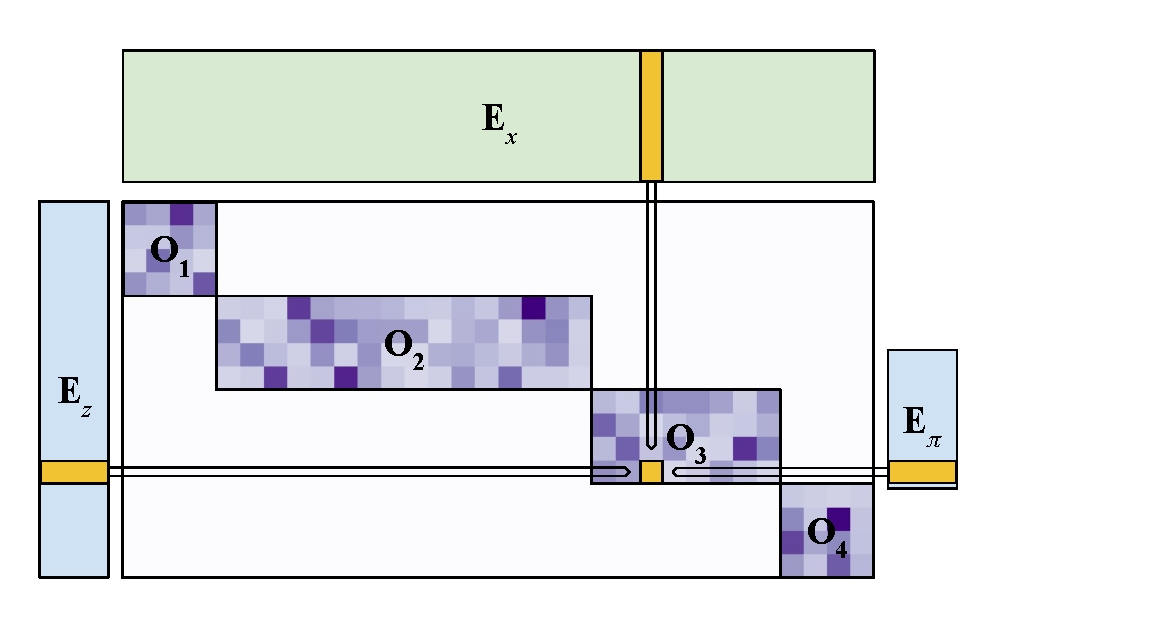
\includegraphics[height=2in]{img/mat.pdf}
\caption{\label{fig:emit}
The transpose of the blocked emission matrix $\mathbf{O}^\top$ generated by the embeddings.
}
\end{figure}

\begin{comment}
We add parameterization constraints to ensure that this property holds.
Specifically, we require that each observed token $x$
only has a fixed number of states $z$ with $p(x \mid z) > 0$.
For each word, we call this support set $\mcC_x \subset \mcZ$.
This yields the following constrained emission distribution:
\begin{equation}
\label{eqn:sparse_emission}
p(x \mid z) \propto \mathbf{1}(z \in \mcC_x)e^{\phi_{xz}}
\end{equation}
\end{comment}

Exact marginalization can be computed as 
\begin{equation}
\label{eqn:sparse_marginalization}
\begin{aligned}
p(\bx) &= \sum_{z_1 \in \mcZ_{x_1}} p(z_1\mid z_0)p(x_1 \mid z_1) \times\\
    &\cdots
    \sum_{z_T \in \mcZ_{x_T}} p(z_T \mid z_{T-1})p(x_T \mid z_T)
\end{aligned}
\end{equation}
This gives a serial complexity of $O(T(|Z|/M)^2)$


%We choose the sets $\mcC_x$ by using the partitions of the
%states $\pi$ and and tokens $\rho$.
%We then have $\mcC_x = \set{z: \pi(z) = \rho(x)}$,
%yielding a computation complexity of $O(Tk^2)$ rather than $O(T|\mcZ|^2)$
%as each partition $|\pi(z)| = k, \forall z$.


\paragraph{Factored Neural Parameterization}

Even with blocked emissions, the scalar parameterization of an HMM grows quadratically
with states due to the transition matrix.
We instead employ a neural parameterization.
The approach is to embed each state in $\cal Z$ ($\mathbf{E}_z \in \mathbb{R}^{|\mcZ| \times h}$),
each token in $\cal X$ ($\mathbf{E}_x \in \mathbb{R}^{|\mcX| \times h}$),
and each partition ($\mathbf{E}_\pi \in \mathbb{R}^{M \times h}$).
From these we can create representations for leaving a state, entering a state,
and emitting a word: 
\[ \mathbf{H}_{\textrm{out}},\mathbf{H}_{\textrm{in}},\mathbf{H}_\textrm{emit}
 = \text{MLP}(\mathbf{E}_\pi, \mathbf{E}_z ) \] 
%which allows the number of parameters to scale linearly with the size of the state space.
%We parameterize the transition and emission distributions using a residual network
%with LayerNorm.
%Let $E\in\mathbb{R}^{v \times h}$ be an embedding matrix,
%where $v$ is the number of embeddings and
%$h$ is the hidden dimension of our neural network.
%Let $E_x \in \mathbb{R}^{|\mcX|\times h}$ be the token embeddings
%and $E_{\textrm{out}},E_{\textrm{in}},E_\textrm{emit}\in \mathbb{R}^{|\mcZ|\times h}$
%be embeddings for leaving, entering, and emitting from a state respectively. 
The HMM distributional parameters are given by,
\begin{equation}
\begin{aligned}
\phi = \mathbf{E}_x \mathbf{H}_\textrm{emit}^\top \;\; 
\psi = \mathbf{H}_\textrm{out} \mathbf{H}_\textrm{in}^\top
\end{aligned}
\end{equation}
where $\phi \in \mathbb{R}^{|X|\times|Z|}$ and
$\psi \in \mathbb{R}^{|Z|\times|Z|}$.
The MLP architecture follows \cite{kim2019cpcfg}.
Please refer to the supplementary material for details. 
This neural parameterization takes $O(h^2 + h|\mcZ| + h|\mcX|)$ parameters.


Note that parameter computation is independent of inference and can be cached at test-time.
%The clean separation between the computation of the distributional parameters and marginal inference
%allows the distributional parameters to be computed and then cached for use in inference.
For training, we compute them once per batch. 
For RNNs and similar models, %transition activations 
emission probabilities must be recomputed for each token. 


\begin{algorithm}[t]
\begin{algorithmic}
\State{Given: block structure and model parameters}
%\Function{ComputeLikelihood}{}
%    \State{Compute parameters $\phi,\psi$ from model parameters}
%    \ForAll{examples $\bx$}
%        \State{Compute log potentials $\Phi = \Call{LogPotentials}{\phi,\psi,\bx,\mcC_x}$}
%        \State{Compute evidence $\log p(\bx) = \Call{Forward}{\Phi}$}
%    \EndFor
%\EndFunction
    \State{Sample block-wise dropout mask $\bb$}
    \State{Compute $\phi,\psi$ ignoring $b_z = 0$}
    \ForAll{batch examples $\bx$}
        \State{ $\Phi = \Call{LogPotentials}{\phi,\psi,\bx,\bb}$}
        \State{$\log p(\bx) = \Call{Forward}{\Phi}$}
    \EndFor
    \State{Update embeddings $\mathbf{E_z, E_x, E_\pi}$ }
\begin{comment}
\Function{LogPotentials}{}
    \State{Given sequence $\bx = \langle x_1,\ldots,x_T \rangle$,
    constraints $\mcC_x$ with $|\mcC_x| = k$,
    transition parameters $\psi$,
    and emission parameters $\phi$}
    \State{Initialize $\Phi \in \mathbb{R}^{T \times k \times k} = 0$}
    \ForAll{$t\in \set{1,\ldots,T}$}
        \State{Set $\Phi[t,:,:] += \psi[x]$}
        \State{Set $\Phi[t,:,:] += \psi[x]$}
    \EndFor
    \State \Return meh \Comment{$O(1)$}
\EndFunction
\Function{Forward}{}
    \For{meh}
        \State{meh}
    \EndFor
    \State \Return meh \Comment{$O(1)$}
\EndFunction
\end{comment}
\end{algorithmic}
\caption{
\label{fig:algo}
VL-HMM Training
}
\end{algorithm}


\paragraph{Dropout as State Reduction}

%Even with a factored parameterization,
%the very large state space of the model makes it possible for the model to use states to
%memorize training patterns.

To encourage generalization through distributed state usage, we introduce dropout to the model. 
We propose a form of HMM state dropout that removes states from use entirely,
which has the added benefit of speeding up inference.

%This forces the model to use different states while also leading to efficiency improvements
%for computing parameterization and inference. 

%Recall distributional parameters of the emission matrix
%$\phi \in \mathbb{R}^{|\mcX|\times|\mcZ|}$
%and the emission sparsity constraints which associate each token $x$
%with a set of states $\mcC_x$.

State dropout acts on each emission block $\mathbf{O}_1 \ldots \mathbf{O}_M$ independently.
Recall each block has $|{\cal Z}| / M$ columns.
For each, we sample a binary dropout mask by sampling
$ \lambda_{\text{drop}} \times(|{\cal Z}| / M)$ dropped row indices uniformly without replacement.
We concatenate these to a global vector $\mathbf{b}$, which, along with the previous constraints,  ensures,
\begin{equation}
\label{eqn:state_dropout}
p(x \mid z) \propto b_{z}1(z \in \mcZ_x)e^{\phi_{xz}}
\end{equation}

State dropout gives a larger practical speed up for both parameter computation and inference.
For a dropout factor of $0.5$ we get a $4\times$ speed improvement for both,
due to reduction of possible transitions.
This structured dropout is also easier to exploit on GPU,
since it maintains block structure with fixed-height.


%Performing marginal inference with state dropout allows us to skip states that are removed 

%Additionally, we do not need to compute the parameters of the
%transition and emission distributions that have been dropped. 
%This reduces the cost of computing $\phi$ and $\psi$ from
%$O(|\mcZ|^2+|\mcZ||\mcX|)$ to $n^2 + n|\mcX|$.


%We utilize the constraint sets induced by $\pi$ and $\rho$
%to ensure that exactly $n$ states remain in each constraint set $\mcC_x$ after applying dropout.
%This is accomplished by subsampling $n$ states from each partition in the preimage of $\pi$,
%which preserves the block structure observed in Fig.~\ref{fig:trellis}
%and allows the number of outgoing edges at each timestep to remain equal to $n$.

%requires $O(Tn^2)$ computation,
%where $n = \max_x \left|\set{z:b_z=1,z \in \mcC_x}\right|$.


%Although a neural parameterization has empirically been shown to find good optima,
%it requires that the distributional parameters be %recomputed every time the
%model parameters are updated.
%This entails running a neural network $O(|\mcZ| + |\mcX|)$ times 
%at every iteration of gradient descent.


\section{HMM Language models}
\label{sec:experiments}
In this section we provide further details on the application
of the methods described in the previous section
to word-level language modeling,
where the tokens $\bx$ correspond to the words
$\bw = \langle w_1,\ldots,w_T \rangle$ in a sentence.
We thus learn a model over words and states
$p(\bw,\bz) = \prod_t p(w_t\mid z_t)p(z_t \mid z_{t-1})$.

\paragraph{State and word partitions}
We use Brown clusters \citep{brown1992,liang2005brown} to construct the state and word partitions.
Brown clusters are obtained by assigning every token type in $\mcX$ a state in a HMM,
then states are merged until a desired number of states $M$ is reached.
Importantly, every word is emit by only a single state, giving us the 
word partitions $\mcX_m$.
We then clone the states of the Brown HMM $|\mcZ|/M$ times to obtain the $\mcZ_x$.

\subsection{Datasets}
We evaluate on the \texttt{Penn Treebank} \citep{ptb}
and \texttt{wikitext2} \citep{wikitext} datasets.
\texttt{Penn Treebank} contains 929k tokens in the training corpus,
with a vocabulary size of 10k.
We use the preprocessing from \citet{mikolov-2011},
which lowercases all words and substitutes words outside of the vocabulary with unks. 
\texttt{Wikitext2} contains 2M tokens in the training corpus,
with a vocabulary size of 33k.
Casing is preserved, and all words outside the vocab are replaced with the unk token.
Both datasets contain inter-sentence dependencies,
due to the use of documents consisting of more than a single sentence.

We construct the Brown clusters on the training portions of both datasets.
As baselines, we train a 5-gram model \citep{kenlm},
a feedforward model with 256 hidden dimensions,
and a 2-layer LSTM with 256 hidden dimension.
We compare these models with an HMM that considers 256 latent states
at every timestep at test time.

\begin{comment}
\paragraph{Implementation}
We train two-layer LSTM recurrent neural networks with 256 units,
as well as two-layer feed-forward neural networks with 256 units.
The HMMs we train follow the sparsity constraints outlined in the previous
section with a dropout rate of 0.5,
and we vary the total number of states as well as states per word.
We optimize all models with AdamW \citep{adamw}.

We experimented with a couple batching strategies:
On \texttt{Penn Treebank},
the first strategy discarded the inter-sentence dependencies and shuffled all sentences,
and the second treated the corpus as a single flat document without shuffling.
On \texttt{Wikitext2}, we either shuffled at the document level or treated the corpus as a
single document.
Prior work on both corpuses treated the corpora as single documents.

See Appendix \ref{sec:hyperparams} for the hyperparameters for all models.
\end{comment}

\section{Results}
%\subsection{Language Modeling}
% Tone: Made a lot of progress, and there is even more room for improvement.
% Main avenue for improvement: emission constraints.
We report perplexities 
for \texttt{Penn Treebank} in Table \ref{tbl:ptb-ppl}
and for \texttt{Wikitext-2} in Table \ref{tbl:wt2-ppl}.

On \texttt{Penn Treebank}, we see in Tbl.~\ref{tbl:ptb-ppl}
that a 32k state HMM is able to outperform the n-gram models
as reported by \citet{mikolov2012rnn}, achieving a test perplexity of
115.8 versus 141.2 respectively.

We also find that the 32k state HMM vastly outperforms the vanilla HMM results from \citet{buys2018hmm},
which achieved a validation perplexity of 284.6
\footnote{\citet{buys2018hmm} did not report test perplexity in their experiments.}
versus the 32k state HMM at 125.0.
The 32k state HMM outperforms their HMM extension, which achieves a
validation perplexity of 142.3 by relaxing various HMM assumptions
to more closely resemble an RNN.

However, we find that the HMM underperforms RNN-based models.
The baseline 2-layer 256 dim LSTM achieves 88.8 test perplexity,
beating the HMM by 27 ppl.
This trend persists in \texttt{Wikitext-2},
with the HMM outperforming the 5-gram model at {\color{red}FILL IN}
and 210.9 perplexity respectively.

\begin{comment}
Since the HMMs require parameters linear in the number of hidden states,
we find that the performance of the HMMs scales poorly compared to the other models
which only require parameters that scale linearly with the vocbaulary size.
Although representing and summing over the hidden states
allows us to explicitly capture uncertainty in the hidden state,
it proves to be a limiting factor in terms of performance.
\end{comment}

In the remainder of this section we ablate and analyze the HMMs on \texttt{Penn Treebank}.


\begin{table*}[!t]
\centering
\begin{tabular}{llll}
\toprule
Model & Num Params & Valid PPL & Test PPL\\
\midrule
KN-5 \citep{mikolov2012rnn}  & 2M & - & 141.2\\
%KN-5 + cache \citep{mikolov2012rnn}  & 2M & - & 125.7\\
RNN \citep{mikolov2012rnn}  & 2M & - & 124.7\\
Medium LSTM \citep{zaremba2014lstm} & 20M & 86.2 & 82.7\\
Large LSTM \citep{zaremba2014lstm} & 66M & 82.2 & 78.4\\
AWD-LSTM \citep{merity2017awdlstm} & 24M & 60.0 & 57.3\\
%AWD-LSTM + cache \citep{merity2017awdlstm} & 24M & 53.9 & 52.8\\
%KN-5 & 2.2M & 161.3 & 157.2\\
HMM \citep{buys2018hmm} & 10M & 284.6 & -\\
HMM + sigmoid + RNN emit \citep{buys2018hmm} & 10M & 142.3 & -\\
\midrule
256 dim FF 5-gram  & 2.9M     & 159.9      & 152.0  \\
2 layer 256 dim LSTM  & 3.6M     & 93.6       & 88.8   \\
32k state HMM   & 7.7M     & 125.0      & 115.8  \\
\bottomrule
\end{tabular}
\caption{\label{tbl:ptb-ppl}
Perplexities on the \texttt{Penn Treebank} dataset.
The bottom section shows results for models 
with comparable computational cost.
In particular, we compare models that have the same 
asymptotic inference cost: linear in
the length of a sequence and quadratic in the hidden
dimension.
This is $h=256$ for the FF model and LSTM
and $|\mcZ| = 256$ for the HMM.
}
\end{table*}

\begin{table*}[!t]
\centering
\begin{tabular}{llll}
\toprule
Model & Num Params & Valid PPL & Test PPL\\
\midrule
AWD-LSTM \citep{merity2017awdlstm} & 33M & 68.6 & 65.8\\
AWD-LSTM-MoS \citep{mos} & 35M & 63.9 & 61.5\\
AWD-LSTM-DOC \citep{awddoc} & 37M & 60.3 & 58.0\\
KN-5              & 5.7M       & 248.7 & 234.3\\
\midrule
256 dim FF 5-gram        & 8.8M    & 210.9  & 195.0\\
2 layer 256 dim LSTM     & 9.6M    & 124.5  & 117.5\\
%32k state HMM (no fac)   & 17.3M   & 166.7  & -\\
32k state HMM            & 13.7M   & -      & -\\
\bottomrule
\end{tabular}
\caption{\label{tbl:wt2-ppl}
Single model perplexities on the \texttt{Wikitext-2} dataset.
The bottom shows results for the models with 
similar computation cost, using the same
hyperparameters applied to \texttt{Penn Treebank}.
}
\end{table*}

\paragraph{Number of states}
In Tbl.~\ref{tbl:states-ablation} we examine the effect of the 
number of states on perplexity.
We find that performance continuously improves as we increase
the size of the state space, up until we reach 65k states.
It is possible that at 65k states, we are bottlenecked by
other aspects of the model, such as the expressive power
or learnability of the neural parameterization. 
%Due to GPU memory constraints, we were unable to further
%explore larger parameterizations, both 
%in terms of the dimension of the neural components as well as 
%the size of the state space.
However, we note that increasing the dimension of the neural component from 256 to
512 dimensions with $|\mcZ| = 32,768$ total states did not improve performance.
Another hypothesis is that the marginal gains in likelihood
decreases as we continue to increase the size of the state space.

\begin{figure}[!t]
\centering
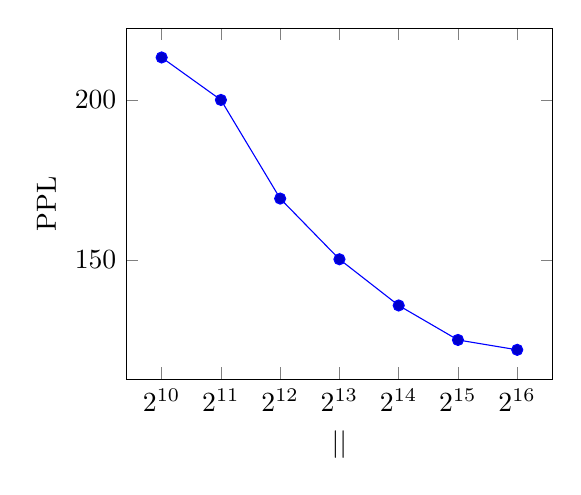
\begin{tikzpicture}
\begin{axis}[
    xlabel=$|\mcZ|$,
    ylabel=PPL,
    xmode=log,
    log basis x={2},
    xtick={},
    width=7cm,
]
  \addplot plot coordinates {
    (1024,  213.25)
    (2048,  199.98)
    (4096,  169.18)
    (8192,  150.22)
    (16384, 135.79)
    (32768, 125.02)
    (65536, 121.93)
};
\end{axis}
\end{tikzpicture}
\caption{\label{tbl:states-ablation}
Perplexities on the \texttt{Penn Treebank} dataset
as a function of the state size $|\mcZ|$.
We hold the emission constraints fixed using 128 Brown clusters,
and state dropout at 0.5.
}
\end{figure}

\begin{table}[h]
\centering
\begin{tabular}{lllll}
\toprule
Constraint & $|\mcZ|$ & $|\mcC_x|$ & $m$ & Val PPL\\
\midrule
Brown & 16384 & 512 & 32  & 137\\
Brown & 16384 & 256 & 64  & 138\\
Brown & 16384 & 128 & 128 & 134\\
Brown & 16384 & 64  & 256 & 136\\
\midrule
None  & 1024 & - & - & 180\\
Brown & 1024 & 256 & 4 & 182\\
Brown & 1024 & 128 & 8 & 194\\
\midrule
Uniform    & 8192    & 128    & -   & 150\\
Brown      & 8192    & 128    & 64  & 142\\
Uniform    & 16384   & 128    & -   & 146\\
Brown      & 16384   & 128    & 128 & 136\\
\bottomrule
\end{tabular}
\caption{\label{tbl:constraint-ablation}
Perplexities on the \texttt{Penn Treebank} dataset.
We ablate the effect of the number of Brown clusters,
examine whether there may be a drop in performance due to the emission sparsity constraint,
and compare the Brown cluster constraint to a uniform baseline.
All models have 0.5 state dropout, except for the 1k state HMMs,
which have no dropout.
We use $m$ to indicate the number of clusters.
}
\end{table}

\paragraph{Emission constraint ablation}
We next analyze the effect of the emission constraint and dropout on performance.
We fix the total number of states at 16k 
and vary the emission constraints and dropout rate.
In the top section of Tbl.~\ref{tbl:constraint-ablation},
we find that the performance is
insensitive to the number of Brown clusters at 16k states.
However, in the middle section,
the model is sensitive to the number of Brown clusters
at 1k total states.
The 1k state HMM with 4 Brown clusters matches the unconstrained 1k state HMM,
while the HMM with 8 Brown clusters underperforms.
This implies that there may be a loss in performance due to the emission constraints.

We additionally compare the partition induced by Brown clustering with a uniform
constraint that samples each $\mcC_x$ of size $n$
independently and uniformly from all subsets of $\mcC$.
This foregoes a partitioning, which makes it difficult to apply state dropout.
We therefore apply a version of dropout that does not have block structure
and zeroes out elements of the transition matrix randomly.
In the bottom section of Tbl.~\ref{tbl:constraint-ablation},
we find that models with uniform constraints
are consistently outperformed by models with Brown cluster constraints
as measured by validation perplexity.
The models with uniform constraints also had poor validation perplexities
despite better training perplexities, a symptom of overfitting.

In conclusion,
we find the Brown cluster emission constraints to achieve reasonable performance
in HMMs with large state spaces.
We also observe that model performance is sensitive to the emission constraints,
motivating future work towards exploring learning emission constraints
while keeping inference tractable. 


\paragraph{Dropout and parameterization ablation}
We ablate state dropout and model parameterization in Tbl.~\ref{tbl:dropout-param-ablation}.
We find that state dropout results in both an improvement in perplexity
and a large improvement in time per epoch.
The train-val gap for the model without state dropout was much larger than 
the model with dropout, highlighting the effectiveness of state dropout as regularization.

The scalar parameterization, which was run with 0.5 state dropout,
has a massive number of model parameters at 423M, compared to the
neural parameterization with 5.6M parameters.
Although the neural and scalar parameterizations reach a similar training perplexity,
the neural model generalizes better on validation.

We additionally ablate the factored state embeddings,
and find that the performance of state embeddings with
independent parameters is similar to a model with factored embeddings.
We additionally found that if the number of clusters is too small
(i.e. 64 or 32 as opposed to 128)
while keeping the total number of hidden states fixed to 16k,
performance on validation drops to 143 perplexity.

\begin{table*}[!t]
\centering
\begin{tabular}{lllll}
\toprule
Model                           & Num params & Train PPL & Val PPL & Time per epoch (s)\\
\midrule
16384 state HMM                 & 5.6M       & 122    & 136  & 159\\
\quad - dropout                 & 5.6M       & 89     & 145  & 363\\
\quad - state emb factorization & 7.2M       & 115    & 134  & 142\\
\quad - neural parameterization & 423M       & 119    & 169 & 520
\footnote{The scalar parameterization should be faster per epoch than the
neural parameterization. We attribute this slowdown
to the speed of indexing in PyTorch.
When working with dropout
the neural parameterization computes subsets
of $\phi$ and $\psi$ lazily via a matmul,
whereas the scalar parameterization already has $\phi$ and $\psi$
available but must index into them to obtain the
un-dropped values.}\\
\bottomrule
\end{tabular}
\caption{\label{tbl:dropout-param-ablation}
We report perplexities on the \texttt{Penn Treebank} dataset
for a 16k state HMM with 0.5 state dropout and 128 Brown clusters, and ablate
dropout and the neural parameterization one at a time.
}
\end{table*}


\begin{comment}
\subsection{Part-of-Speech Tagging}

\begin{table*}[!t]
\centering
\begin{tabular}{llll}
\toprule
Model                               & Num params & Valid Acc & Test Acc\\
\midrule
BRNN \citep{ma2016crf}              & -          & 96.56     & 96.76    \\ 
BLSTM \citep{ma2016crf}             & -          & 96.88     & 96.93    \\ 
BLSTM + CNN \citep{ma2016crf}       & -          & 97.34     & 97.33    \\ 
BLSTM + CNN + CRF \citep{ma2016crf} & -          & 97.46     & 97.55    \\ 
\midrule
HMM                                 & 19M        & 96.25     & 96.50    \\
HMM + CNN Emit                      & 9M         & 96.73     & 96.95    \\
\bottomrule
\end{tabular}
\caption{\label{tbl:pos}
Tagging accuracies on the Wall Street Journal (WSJ) portion of the
\texttt{Penn Treebank}.
We use a HMM with 32k states and 0.5 state dropout.
}
\end{table*}

We find in Tbl.~\ref{tbl:pos} that the HMM outperforms the BRNN and BLSTM baselines
of \citep{ma2016crf}, but underperforms the BLSTM with CNN and CRF variants.
Additionally,
we found that incorporating pretrained embeddings in the HMMs did not improve performance.
{\color{red} NEED ERROR ANALYSIS}
\end{comment}

\section{Conclusion}

\bibliographystyle{acl_natbib}
\bibliography{anthology,emnlp2020}

\appendix

\section{Hyperparameters}
\label{sec:hyperparams}
For \texttt{Penn Treebank} and \texttt{Wikitext-2}, we had the following baselines:
a two layer feedforward 5-gram model and a two layer LSTM.
The feedforward model is given by the following:
\begin{equation}
\begin{aligned}
p(w_t \mid w_{<t})
&= W_x\textrm{ReLU}(\textrm{Conv}(\bw_{t-4:t-1}))
\end{aligned}
\end{equation}
where $\bw$ gives the word embeddings and $W_x\in\mathbb{R}^{|\mcX|\times h}$ is weight-tied to the embeddings.

For the feedforward model we use a batch size of 128 and a bptt length of 64, as we found the model needed a larger batch size to train.
For the LSTM, we use a batch size of 16 and a BPTT length of 32.
For both baseline models we use a learning rate of 1e-3 and a dropout rate of 0.3 on the activations in the model.
Both models use a hidden dimension of 256 throughout.
These same hyperparameters were applied on both \texttt{Penn Treebank} and \texttt{Wikitext-2}.

For the HMMs also use a batch size of 16 and a BPTT length of 32. We use state dropout with a rate of 0.5. We use a learning rate of 1e-2 for \texttt{Penn Treebank}, and a learning rate of 1e-3 for \texttt{Wikitext-2}.

\section{HMM Parameterization}
The HMMs use the following residual network:
\begin{equation}
\label{eqn:res}
\begin{aligned}
f_i(E) &= g_i(\textrm{ReLU}(EW_{i1}))\\
g_i(D) &= \textrm{LayerNorm}(\textrm{ReLU}(DW_{i2}) + D)
\end{aligned}
\end{equation}
with $i \in \set{\textrm{out},\textrm{in},\textrm{emit}}$.
We then have
\begin{equation}
\begin{aligned}
\mathbf{H}_\textrm{out} &= f_\textrm{out}(f_o([\mathbb{E}_\pi,\mathbb{E}_z]))\\
\mathbf{H}_\textrm{in} &= f_\textrm{in}(f_i([\mathbb{E}_\pi,\mathbb{E}_z]))\\
\mathbf{H}_\textrm{emit} &= f_\textrm{emit}(f_e([\mathbb{E}_\pi,\mathbb{E}_z]))
\end{aligned}
\end{equation}
where we have further have another residual network to combine $\mathbb{E}_\pi$ and $\mathbb{E}_z$ for each set of embeddings.

\section{Supplemental Material}
\label{sec:supplemental}
\end{document}
